\lecture[Zusammenhang, Wegzusammenhang. Bilder (weg-) zusammenhängender Räume. Lemma von Urysohn.]{Di 11 Mai 2021 12:16}{Zusammenhang}

\section{Zusammenhang, Wegzusammenhang}

\begin{definition}[Zusammenhang]\label{def:zusammenhang}
    Ein topologischer Raum heißt \vocab[Topologischer Raum!zusammenhängend]{zusammenhängend}, wenn er sich \underline{nicht} in zwei nichtleere, disjunkte, offene Teilmengen zerlegen lässt. 
\end{definition}

\begin{dlemma}[Offen-abgeschlossene-Mengen]\label{lm:raum-ist-zusammenhängend-gdw-offen-abgeschlossene-mengen-sind-trivial}
    Ein Raum ist zusammenhängend, wenn die leere Menge und der gesamte Raum die einzigen Teilmengen von $X$ sind, die offen und abgeschlossen sind, d.h.
     \[
    \not \exists  A\subset X, A\neq \emptyset,X \colon \quad A \text{ offen und abgeschlossen}
    .\] 
\end{dlemma}

\begin{proof*}
    Klar.
\end{proof*}

\begin{remark}
    $X$ ist nicht zusammenhängend, genau dann, wenn  $X \cong X_1 \coprod X_2$ eine disjunkte Vereinigung von 2 Räumen $X_1,X_2\neq \emptyset$ ist.
\end{remark}

\begin{example}
    \begin{enumerate}[1)]
        \item $\R\setminus \left \{0\right\}  = (-\infty,0) \cup (0,\infty)$ und $(-\infty,0),(0,\infty)$ sind offen, disjunkt und nicht leer, also ist $\R\setminus \left \{0\right\} $ \underline{nicht} zusammenhängend. 
        \item Betrachte $\Q\subset \R$ mit der Unterraumtopologie. Dann ist
            \[
                \Q = (\Q \cap (-\infty,\sqrt{2})) \cup (\Q \cap (\sqrt{2},\infty))  
            .\] 
            eine Zerlegung in offene, disjunkte, nichtleere Mengen, also ist auch $\Q$ nicht zusammenhängend.
    \end{enumerate}
\end{example}

\begin{remark*}
    Es ist meistens einfacher, zu zeigen, dass ein Raum nicht zusammenhängend ist, die Gegenrichtung erweist sich als schwerer. Deswegen folgender
\end{remark*}

\begin{theorem}[Einheitsintervall]\label{thm:einheitsintervall-ist-zusammenhängend}
    Das Intervall $[0,1]$ ist zusammenhängend.
\end{theorem}

\begin{proof}
    Nimm gegenteilig an, dass $[0,1]$ nicht zusammenhängend ist, schreibe also  $[0,1] = A \cup B$ mit $A,B \neq \emptyset$, offen und disjunkt. OBdA sei $0\in A$. Wegen $B\neq \emptyset$ gibt es $t:= \inf B$. Da  $t$ abgeschlossen (weil  $A$ offen!), ist  $t\in B$, also folgt $[0,t) \subset A$. Aber jede Umgebung von $t\in B$ schneidet $[0,t)$, also  $A$, \contra, weil  $A\cap B = \emptyset$.
\end{proof}

\begin{ddefinition}[Weg]\label{def:weg}
    Sei $X$ ein topologischer Raum und $x,y\in X$. Ein  \vocab{Weg} von $x$ nach $y$ ist eine stetige Funktion $w: [0,1] \to  X$, sodass $w(0) =x$ und  $w(1) = y$.
\end{ddefinition}

\begin{definition}[Wegzusammenhang]\label{def:wegzusammenhang}
    Ein topologischer Raum $X$ heißt  \vocab{wegzusammenhängend}, falls für je zwei Punkte $x,y\in X$ ein \vocab{Weg} von $x$ nach  $y$ existiert.
\end{definition}

\begin{example}
    \begin{enumerate}[1)]
        \item     Die Mengen $(a,b), [a,b), (a,b]$ und $\R$ sind alle wegzusammenhängend. Definiere hierzu
        \begin{equation*}
        w: \left| \begin{array}{c c l} 
            [0,1] & \longrightarrow & \R \\
            t & \longmapsto &  ty + (1-t)x
        \end{array} \right.
    \end{equation*}
   Als Verknüpfung stetiger Funktionen ist $t$ stetig, und wir sehen leicht, dass  $0 \mapsto x, 1 \mapsto y$. 
   \item $\R^n, n\geq 0$ ist wegzusammenhängend. Dazu betrachte vorherige Abbildung auf den einzelnen Komponenten
   \item $\R^n \setminus \left \{0\right\} , n\geq 2$ ist wegzusammenhängend. Seien hierzu $x,y\in \R^n \setminus \left \{0\right\}$.
       \begin{description}
           \item[Fall 1:] Die Strecke von $x$ nach  $y$ liegt in  $\R^n \setminus \left \{0\right\}$. Dann betrachten wir wieder die Abbildung aus 1) und sind fertig.
           \item[Fall 2:] Die Strecke trifft die $0$. Wähle dann einen dritten Punkt $z$, der nicht auf der Geraden durch $x,y$ liegt. Dann gibt es einen Weg von $x$ nach  $z$ und einen von  $z$ nach  $x$, und die Vereinigung der beiden Wege ist dann ein Weg von  $x$ nach  $y$.
       \end{description}
    \end{enumerate}
\end{example}

\begin{lemma}\label{lm:wegzusammenhang-impliziert-zusammenhang}
    Ist $X$ wegzusammenhängend, so ist  $X$ zusammenhängend.
\end{lemma}

\begin{warning}
    Die Umkehrung von \autoref{lm:wegzusammenhang-impliziert-zusammenhang} gilt im Allgemenien nicht. Siehe hierzu Übungsblatt 5, Aufgabe 1.
\end{warning}

\begin{proof}[Beweis von \autoref{lm:wegzusammenhang-impliziert-zusammenhang}]
    Sei $X$ wegzusammenhängend, und nimm gegenteilig an, dass  $X = U_1 \sqcup U_2$ mit $U_i \subset X$ offen und disjunkt. Sei $x_1 \in U_1, x_2\in U_2$. Dann gibt es einen Weg $w$ von  $x_1$ nach $x_2$, und  wir erhalten
    \[
        w^{-1}(U_1) \cup w^{-1}(U_2) = w^{-1}(U_1\cup U_2) = [0,1]
    .\] 
    Allerdings sind $w^{-1}(U_i)$ offen ($w$ ist stetig), disjunkt ($U_1,U_2$ sind disjunkt) und nicht leer ($0\in w^{-1}(U_1)$, $1\in w^{-1}(U_2)$), also ist $[0,1]$ nicht zusammenhängend. \contra mit \autoref{thm:einheitsintervall-ist-zusammenhängend}.
\end{proof}

\begin{corollary}\label{cor:R-und-R2-sind-nicht-homöomorph}
    $\R$ und $\R^2$ sind nicht homöomorph.
\end{corollary}
\begin{proof}
    Nimm an, es gibt einen solchen Homöomorphismus
        \begin{equation*}
        f: \left| \begin{array}{c c l} 
        \R^2 & \longrightarrow & \R \\
        0 & \longmapsto &  f(0)
        \end{array} \right.
    \end{equation*}
    Dann induziert $f$ auch einen Homöomorphismus $\R^2 \setminus \left \{0\right\} \cong \R \setminus \left \{f(0)\right\} $, allerdings ist $\R^2 \setminus \left \{0\right\} $ wegzusammenhängend, und $\R \setminus \left \{f(0)\right\} $ nicht, \contra.
\end{proof}

\begin{question}
    Sind $\R^n, \R^m$ wegzusammenhängend?
\end{question}

\begin{answer}
    Nein, das gilt natürlich genau dann, wenn $n = m$. Allerdings warten wir mit einem solchen Beweis bis zur algebrasichen Topologie. Siehe hierzu auch 'Invariance of domain', Brower.
\end{answer}
\todo{Referenz}
Ein Versuch für einen ähnlichen Beweis scheitert, weil $\R^2 \setminus \left \{0\right\}$ und $\R^3 \setminus \left \{f(0)\right\} $ beide (weg)zusammenhängend sind. Man könnte nun Versuchen, eine Gerade oder einen Kreis von $\R^2$ zu entfernen, der entsprechende Raum ist dann unzusammenhängend. Es erscheint auch klar, dass $\R^3 \setminus f(\text{Kreis / Gerade})$, allerdings ist ein entsprechender Beweis verhältnismäßig schwer. Die algebraische Topologie wird es uns ermöglichen, das wesentlich einfacher einzusehen.

\begin{remark*}
    Die Frage, ob eine Schleife in $\R^2$ (ein stetiges, injektives Bild von $\mathcal{S}^1$ in $\R^2$) den Raum in zwei Teile zerteilt, ist auch schwerer als man denkt, hierzu siehe 'Jordan curve theorem' (Satz von Jordan-Schönflies).
\end{remark*}
\todo{Referenz}

\begin{comment} %%Unklar, inwiefern das hier ins Skript sollte, war Thema in der Pause.
Zur Motivation der Definition für den Zusammenhang: Man sollte über Zusammenhang eher wie in der Graphentheorie nachdenken.
Das Königsberger Brückenproblem ist gewissermaßen ein 'Urproblem der Topologie'.
\end{comment}

\begin{lemma}[Bilder von zusammenhängenden Räumen]\label{lm:bilder-von-zusammenhängenden-räumen-sind-zusammenhängend}
    Sei $f: X \to  Y$ stetig und surjektiv.
    \begin{enumerate}[1)]
        \item Ist $X$ wegzusammenhängend, so ist  $Y$ wegzusammenhängend.
        \item Ist  $X$ zusammenhängend, so ist $Y$ zusammenhängend.
    \end{enumerate}
\end{lemma}
\begin{proof}
    \begin{enumerate}[1)]
        \item Seien $y_1,y_2\in Y$ beliebig. Da $f$ surjektiv ist, finden wir  $x_1,x_2\in X$ mit $f(x_1) = y_1$, $f(x_2=y_2)$. Nun finden wir wegen Wegzusammenhang von $X$ einen Weg  $w: [0,1] \to X$ mit $w(0) = x_1$ und $w(1) = x_2$. Dann ist die Verknüpfung
                \begin{equation*}
                f \circ  w: \left| \begin{array}{c c l} 
                    [0,1] & \longrightarrow & Y \\
                    0 & \longmapsto &  f(x_1) = y_1 \\
                    1 & \longmapsto & f(x_2) = y_2
                \end{array} \right.
            \end{equation*}
            ein Weg von $y_1$ nach $y_2$, also ist $Y$ wegzusammenhängend.
        \item Nimm an, dass $Y$ nicht zusammenhängend ist, also gibt es  $U_1,U_2\neq \emptyset$ offen und disjunkt mit $Y = U_1 \cup U_2$. Dann ist auch
            \[
                X = f^{-1}(Y) = f^{-1}(U_1\cup U_2) = f^{-1}(U_1) \cup f^{-1}(U_2)
            .\] 
            und $f^{-1}(U_i)$ sind offen, disjunkt und nichtleer, weil $f$ surjektiv ist. Also ist $X$ nicht zusammenhängend, \contra.
    \end{enumerate}
\end{proof}
\begin{example}
    Die Sphäre $S^n, n\geq 1$ ist wegzusammenhängend. Hierzu stellen wir fest, dass
    \[
        \R^n \setminus \left \{0\right\}  \cong S^{n-1}\times \R \stackrel{\text{Projektion}}{\longrightarrow} S^{n-1}
    .\] 
und wir wissen schon, dass $\R^n \setminus \left \{0\right\}$ wegzusammenhängend ist, also auch $S^{n-1}$.
\[
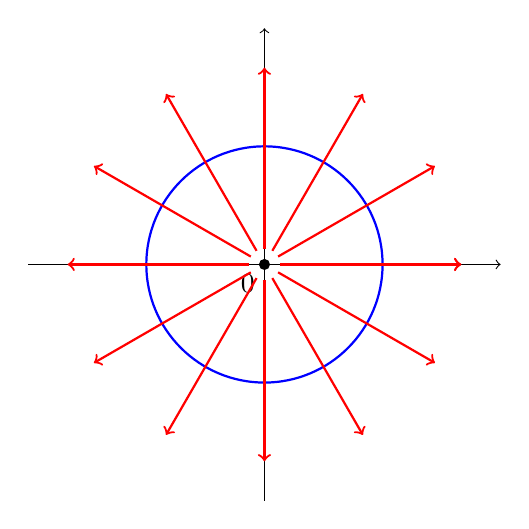
\begin{tikzpicture}
    \draw[->] (-3,0) -- (3,0);
    \draw[->] (0,-3) -- (0,3) node[midway, anchor = north east] {$0$};
    \fill (0,0) circle (2pt);
    \draw[blue, thick] (0,0) circle (1.5);
    \foreach \x in {0,...,12} {
        \draw[red,thick,->] (\x*30:0.2) -- (\x*30:2.5);
    }
\end{tikzpicture}
.\] 
\end{example}

\begin{remark}
    Jede sternförmige Teilmenge von $\R^n$ ist wegzusammenhängend. Hierzu
    \[
    \text{konvex } \implies \text{ sternförmig } \implies \text{wegzusammenhängend}
    .\] 
\end{remark}


\section{Lemma von Urysohn}

\begin{theorem}[Urysohn'sches Lemma]\label{thm:urysohn}
    Sei $X$ ein normaler topologischer Raum. Seien  $A,B\subset X$ abegschlossen und disjunkt. Dann existiert eine stetige Abbildung $f: X \to  [0,1]$, sodass $f\mid _A \equiv 0 $ und $f\mid _{B} \equiv  1$.
\end{theorem}
\todo{Grafik}

\begin{lemma}\label{lm:stetige-abbildung-durch-familie-von-rationalen-offenen-mengen}
    Sei $X$ ein topologischer Raum, sodass für jedes $r\in [0,1]\cap \Q$ offene $V_r \subset X$, sodass $r < r' \implies \overline{V_r} \subset V_{r'}$. Dann existiert eine stetige Abbildung $f: X \to  [0,1]$, sodass $f(x) = 0$ für  $x\in V_0$ und $f(x) = 1$ für  $x\not\in V_1$.
\end{lemma}
\begin{proof}
    Definiere
        \begin{equation*}
        f: \left| \begin{array}{c c l} 
            X & \longrightarrow & [0,1] \\
            x & \longmapsto &  \begin{cases}
                1 & x\not\in V_1 \\
            \inf \left \{r \mid  x\in V_r\right\} & x\not\in V_1
            \end{cases}
        \end{array} \right.
    \end{equation*}
    Die Eigenschaften $f\mid _{V_0} \equiv 0$ und $f\mid _{X \setminus V_i} \equiv  1$ sind sofort klar. Es bleibt zu zeigen, dass $f$ stetig ist. Da
    \[
        \mathcal{S} := \left \{[0,a) \mid  a\in [0,1]\right\}  \cup \left \{(a,1] \mid  a\in [0,1]\right\} 
    .\] 
    eine Subbasis der Topologie auf $[0,1]$ ist, genügt es, Stetigkeit auf  $\mathcal{S}$ zu prüfen. Sei
    \begin{IEEEeqnarray*}{rCl}
        x\in f^{-1}([0,a)) & \iff & f(x) < a \leq  1 \\
                           & \stackrel{\text{Def von $f$}}{\iff} &  \inf \left \{r \mid  x\in V_r\right\} <a \\
                           &\stackrel{\Q \text{ ist dicht}}{\iff} & \exists r < a, r\in \Q \colon x\in V_r \\
                           & \iff&  x\in \bigcup_{r<a} V_r 
    \end{IEEEeqnarray*}
    Für den zweiten Typ von Basielementen ist
    \begin{IEEEeqnarray*}{rCl}
        x\in f^{-1}((a,1]) & \iff& \begin{cases}
                x\not\in V_1 &\text{oder} \\
                x\in V_1, a < f(x) = \inf \left \{r\mid x\in V_r\right\}
        \end{cases} \\
                           & \iff  & \exists r'>a, r'\in \Q, x\not\in V_r \\
                           & \stackrel{\overline{V_r} \subset V_{r'}}{\iff}  & \exists r\in \Q, a<r < r', x\not\in \overline{V_r} \\
                           & \iff  & x\in \bigcup_{r>a} \left( X \setminus \overline{V_r} \right)  
    \end{IEEEeqnarray*}
    also ist auch $f^{-1}((a,1])$ eine Vereinigung von offenen Mengen. \\
    Also ist $f$ stetig, wie zu zeigen war.
\end{proof}

\begin{remark*}
    Wir können uns die $V_r$ wie eine Art 'Höhenprofil' oder 'Höhenlienien' vorstellen, die wir in unserem Raum gegeben haben. 
\end{remark*}
